\documentclass[runningheads]{llncs}

\usepackage[utf8]{inputenc}
\usepackage[T1]{fontenc}
\usepackage[romanian]{babel}
\usepackage{graphicx}
\usepackage{hyperref}
\usepackage{array}
\usepackage{listings}
\usepackage{amsmath}
\usepackage{float}
\usepackage{enumitem}
\usepackage{titlesec}

% Reducerea spatiilor pentru subsectiuni si sectiuni
\titlespacing*{\section}{0pt}{6pt plus 1pt minus 1pt}{3pt plus 1pt minus 1pt}
\titlespacing*{\subsection}{0pt}{3pt plus 1pt minus 1pt}{3pt plus 1pt minus 1pt}
\titlespacing*{\subsubsection}{0pt}{2pt plus 1pt minus 1pt}{2pt plus 1pt minus 1pt}

\title{Raport tehnic: Aplicație Client--Server pentru Evaluarea Problemelor de Programare}
\author{Curmei Bianca}
\institute{Facultatea de Informatică, Universitatea "Alexandru Ioan-Cuza" din Iași}

\begin{document}

\maketitle
\thispagestyle{plain}
\pagestyle{plain}

\section*{Introducere}

Acest raport descrie implementarea unei aplicații client--server în limbajul C, folosind socket-uri TCP și un model de concurență bazat pe procese (\texttt{fork()}). Aplicația permite clienților să solicite probleme de programare, să trimită soluții în C și să primească rezultate, calculând automat scorurile în funcție de corectitudinea soluției, timpul de execuție și viteza de trimitere a fișierelor.

\vspace{3mm}

Obiectivele proiectului sunt:
\begin{itemize}[noitemsep, topsep=0pt]
    \item înțelegerea comunicării prin socket-uri TCP;
    \item implementarea unui server concurent folosind \texttt{fork()} pentru mai mulți clienți simultan;
    \item crearea unui protocol simplu de nivel aplicație, bazat pe comenzi text;
    \item evaluarea automată a soluțiilor de programare în C.
\end{itemize}

\vspace{3mm}

Aplicația servește ca prototip pentru o platformă de evaluare automată a participanților la olimpiade de informatică.

\vspace{10mm}

\section{Tehnologii Aplicate}

\subsection{Limbajul de programare}
Proiectul este implementat în \textbf{C}, oferind acces direct la socket-uri, control asupra memoriei și execuției, și integrare ușoară cu scripturi bash pentru compilare și testare.

\vspace{5mm}

\subsection{Protocolul de transport}
Comunicarea dintre client și server se realizează prin \textbf{TCP}, care asigură:
\begin{itemize}[noitemsep, topsep=0pt]
    \item comunicare fiabilă;
    \item garantarea ordinii mesajelor;
    \item menținerea unei conexiuni persistente potrivită pentru dialog interactiv.
\end{itemize}

Serverul ascultă pe portul 5151.

\vspace{5mm}

\subsection{API-ul de socket-uri}
Se utilizează API-ul standard Berkeley Sockets:
\begin{itemize}[noitemsep, topsep=0pt]
    \item \texttt{socket()}, \texttt{bind()}, \texttt{listen()}, \texttt{accept()};
    \item \texttt{connect()}, \texttt{send()}, \texttt{recv()}.
\end{itemize}

\subsection{Modelul de concurență}
Serverul folosește concurență prin procese:
\begin{itemize}[noitemsep, topsep=0pt]
    \item procesul părinte ascultă permanent conexiuni noi;
    \item la acceptarea unui client, se creează un proces copil cu \texttt{fork()};
    \item procesul copil gestionează comunicarea cu clientul: trimiterea problemelor și evaluarea soluțiilor.
\end{itemize}

\vspace{10mm}

\section{Structura Aplicației}

Aplicația este împărțită în două programe principale: \texttt{server} și \texttt{client}, împreună cu scripturi auxiliare pentru compilare și rularea testelor. Structura aplicației și responsabilitățile fiecărui component sunt detaliate mai jos.

\subsection{Structura directoarelor generale}

\begin{verbatim}
problems/
  problem1/
    statement.txt
    tests/
      test1.in, test1.out, ...
submissions/
results/
scripts/
\end{verbatim}

\subsection{Structura Serverului}

\begin{description}[noitemsep, topsep=0pt]
    \item[Fișiere:] 
    \begin{itemize}[noitemsep, topsep=0pt]
        \item \texttt{server.c} - gestionează conexiunile clienților și logica principală;
        \item \texttt{problem\_manager.c/h} - încarcă problemele și testele din directoarele locale;
        \item \texttt{evaluator.c/h} - compilează și rulează soluțiile, calculează scorurile;
        \item \texttt{utils.c/h} - funcții de ajutor pentru trimiterea/primirea mesajelor și prelucrarea inputului;
        \item scripturile \texttt{compile\_solution.sh} și \texttt{run\_tests.sh} pentru compilare și testare automată.
    \end{itemize}
    \item[Funcționalitate:]
    \begin{itemize}[noitemsep, topsep=0pt]
        \item primește conexiuni TCP de la clienți pe portul 5151;
        \item la fiecare client, creează un proces copil (\texttt{fork()}) care gestionează întreaga sesiune;
        \item implementează comenzile: 
        \begin{itemize}[noitemsep, topsep=0pt]
            \item \texttt{GET PROBLEM} - trimite enunțul unei probleme aleatoare;
            \item \texttt{SEND SOLUTION} - primește soluția clientului și o salvează în \texttt{submissions/};
            \item \texttt{GET RESULTS} - calculează și trimite scorul final;
            \item \texttt{GET RANKING} - trimite lista tuturor participanților și scorurile lor;
            \item \texttt{QUIT} - închide conexiunea cu clientul.
        \end{itemize}
    \end{itemize}
\end{description}

\subsection{Structura Clientului}

\begin{description}[noitemsep, topsep=0pt]
    \item[Fișiere:]
    \begin{itemize}[noitemsep, topsep=0pt]
        \item \texttt{client.c} - programul principal pentru interacțiunea utilizatorului;
        \item \texttt{utils.c/h} - funcții utilitare pentru comunicare și prelucrarea inputului.
    \end{itemize}

    \item[Funcționalitate:]
    \begin{itemize}[noitemsep, topsep=0pt]
        \item se conectează la serverul local pe portul 5151;
        \item citește comenzile de la utilizator și le trimite serverului;
        \item afișează răspunsurile serverului: probleme, scoruri, clasament.
    \end{itemize}
\end{description}

\subsection{Diagrama de comunicare}

\begin{figure}[H]
    \centering
    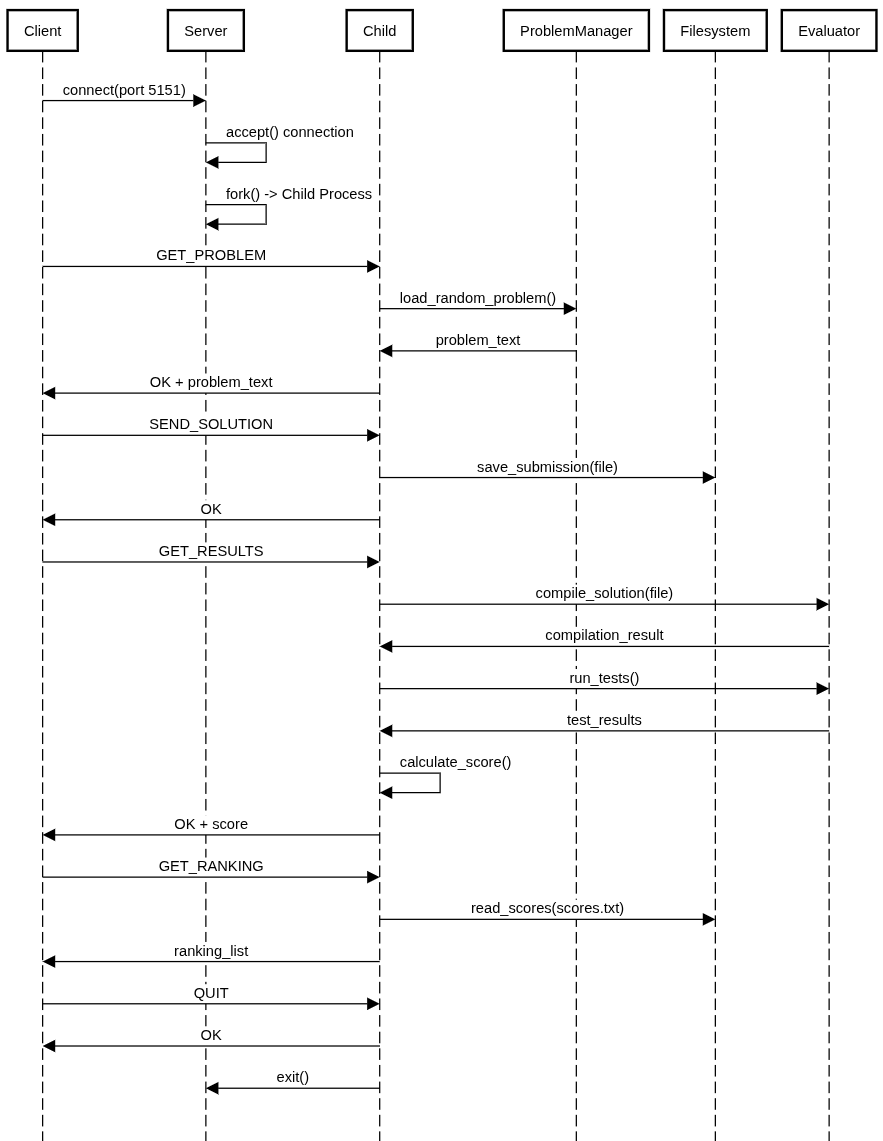
\includegraphics[width=\textwidth]{sequencediagram.png}
    \label{fig:sequencediagram}
\end{figure}

\vspace{10mm}

\noindent
\textbf{Explicație detaliată a diagramei secvențiale:}

\begin{itemize}[noitemsep, topsep=0pt]
    \item \textbf{Conectarea clientului la server:} Clientul inițiază o conexiune TCP către server pe portul 5151. Serverul principal acceptă conexiunea și creează un proces copil folosind \texttt{fork()} pentru a gestiona această sesiune.

    \vspace{5mm}
    
    \item \textbf{Solicitarea unei probleme (\texttt{GET\_PROBLEM}):} Clientul trimite comanda \texttt{GET\_PROBLEM} către procesul copil. Copilul solicită un enunț aleatoriu din modulul \texttt{ProblemManager}, care îl încarcă din directorul \texttt{problems/}. Problema este trimisă clientului împreună cu confirmarea \texttt{OK}.

    \vspace{5mm}
    
    \item \textbf{Trimiterea soluției (\texttt{SEND\_SOLUTION}):} Clientul trimite fișierul sursă al soluției. Procesul copil salvează soluția în directorul \texttt{submissions/} și confirmă primirea cu \texttt{OK}.

    \vspace{5mm}
    
    \item \textbf{Evaluarea rezultatelor (\texttt{GET\_RESULTS}):} Clientul solicită scorul. Copilul compilează soluția folosind modulul \texttt{Evaluator}, rulează testele stocate în directorul problemei, colectează rezultatele și calculează scorul final. Scorul este trimis clientului împreună cu \texttt{OK}.

    \vspace{5mm}
    
    \item \textbf{Obținerea clasamentului (\texttt{GET\_RANKING}):} Clientul solicită clasamentul. Procesul copil citește fișierul \texttt{results/scores.txt}, care conține scorurile tuturor participanților, și trimite lista clientului.

    \vspace{5mm}
    
    \item \textbf{Închiderea conexiunii (\texttt{QUIT}):} Clientul închide sesiunea trimițând comanda \texttt{QUIT}. Procesul copil confirmă cu \texttt{OK} și se termină, eliberând resursele alocate.

    \vspace{5mm}
    
    \item \textbf{Separarea proceselor și modulelor:} Serverul principal rămâne disponibil pentru alte conexiuni, în timp ce fiecare client activ este gestionat independent de un proces copil. Acest model asigură concurență și izolare între sesiunile clienților.
\end{itemize}

\vspace{10mm}

\section{Protocolul de Comunicare}

\subsection{Comenzi client}
\begin{table}[H]  
\centering
\begin{tabular}{|m{3.5cm}|m{8cm}|}
\hline
\textbf{Comandă} & \textbf{Descriere} \\ \hline
GET PROBLEM & Solicită o problemă aleatorie. \\ \hline
SEND SOLUTION & Trimite o soluție în C. \\ \hline
GET RESULTS & Solicită rezultatul evaluării. \\ \hline
GET RANKING & Solicită clasamentul tuturor participanților. \\ \hline
QUIT & Închide conexiunea. \\ \hline
\end{tabular}
\end{table}

\subsection{Răspunsuri server}
\begin{itemize}[noitemsep, topsep=0pt]
    \item \textbf{OK} - comandă procesată cu succes;
    \item \textbf{ERR} - comandă invalidă sau eroare.
\end{itemize}

\vspace{5mm}

\subsection{Exemplu de dialog}
\begin{verbatim}
Client: GET_PROBLEM
Server: OK
Server: Problema 3: Sortare prin interclasare.
Client: SEND_SOLUTION
Server: OK
Client: GET_RESULTS
Server: OK 95
Client: QUIT
Server: OK
\end{verbatim}

\vspace{10mm}

\section{Scenarii de Utilizare}

\subsection{Scenarii de succes}

\textbf{Scenariul 1:} Client cere o problemă și apoi închide conexiunea.
\begin{enumerate}[noitemsep, topsep=0pt]
    \item Clientul se conectează la server.
    \item Trimite \texttt{GET PROBLEM}; serverul răspunde cu \texttt{OK} + problemă.
    \item Trimite \texttt{QUIT}; serverul confirmă cu \texttt{OK}.
    \item Clientul închide conexiunea.
\end{enumerate}

\vspace{5mm}

\textbf{Scenariul 2:} Flux complet.
\begin{enumerate}[noitemsep, topsep=0pt]
    \item Clientul se conectează.
    \item Trimite \texttt{GET PROBLEM}; serverul trimite problema.
    \item Trimite \texttt{SEND SOLUTION}; serverul confirmă.
    \item Trimite \texttt{GET RESULTS}; serverul trimite scorul calculat.
    \item Trimite \texttt{GET RANKING}; serverul trimite clasamentul.
    \item Trimite \texttt{QUIT}; serverul confirmă.
\end{enumerate}

\vspace{5mm}

\textbf{Scenariul 3:} Mai mulți clienți simultan.
\begin{enumerate}[noitemsep, topsep=0pt]
    \item Mai mulți clienți se conectează.
    \item \texttt{accept()} creează socket dedicat fiecărui client.
    \item \texttt{fork()} creează un proces copil per client.
    \item Fiecare proces copil gestionează independent propriul client.
\end{enumerate}

\vspace{15mm}

\subsection{Scenarii de eșec}

\textbf{Scenariul 1:} Comandă invalidă.
\begin{enumerate}[noitemsep, topsep=0pt]
    \item Clientul trimite \texttt{HELLO}.
    \item Serverul răspunde cu \texttt{ERR}.
    \item Clientul decide să încerce din nou sau să închidă conexiunea.
\end{enumerate}

\vspace{5mm}

\textbf{Scenariul 2:} Serverul se închide brusc.
\begin{enumerate}[noitemsep, topsep=0pt]
    \item Clientul este conectat.
    \item Serverul se oprește neașteptat.
    \item Clientul trimite o comandă și apare eroare de citire/scriere.
    \item Clientul închide aplicația.
\end{enumerate}

\vspace{5mm}

\textbf{Scenariul 3:} Portul 5151 este ocupat.
\begin{enumerate}[noitemsep, topsep=0pt]
    \item \texttt{bind()} eșuează.
    \item Serverul afișează eroare și se închide.
    \item Clientul vede \texttt{connection refused}.
\end{enumerate}

\vspace{10mm}

\section{Concluzii}

Aplicația demonstrează modul de funcționare al unui sistem client--server bazat pe TCP și concurență prin procese. Codul este simplu, robust și ușor de extins.

\vspace{3mm}

Posibile îmbunătățiri:
\begin{itemize}[noitemsep, topsep=0pt]
    \item comunicare criptată TLS pentru securitate;
    \item trecerea la model concurent pe thread-uri sau epoll pentru scalabilitate mare;
    \item definirea unui protocol structurat (JSON/XML) pentru extensibilitate si interoperabilitate;
    \item interfata grafica sau web pentru utilizatori
\end{itemize}

\vspace{10mm}

\section*{Referințe}

\begin{enumerate}[noitemsep, topsep=0pt]
    \item Documentația Linux: \texttt{man socket}, \texttt{man bind}, \texttt{man listen}.
    \item Documentația \texttt{fork(2)}.
    \item Springer LNCS Author Guidelines: \url{https://www.springer.com/gp/computer-science/lncs/conference-proceedings-guidelines}.
    \item Pagina cursului Rețele de Calculatoare: \url{https://edu.info.uaic.ro/computer-networks/cursullaboratorul.php}.
\end{enumerate}

\end{document}

